%Miriam Clustering
The first question was: is it possible without knowing the social classes to reproduce them based on the movement data. Therefore we wanted to look for clusters and compare those with the strata. Also we had a look if the possibly found clusters have special properties.
\subsubsection{Clustering with RapidMiner}

RapidMiner has different Modules for Clustering already implemented. We decided to concentrate on the k-means clustering algorithm.
\begin{figure}[!htbp]
\centering
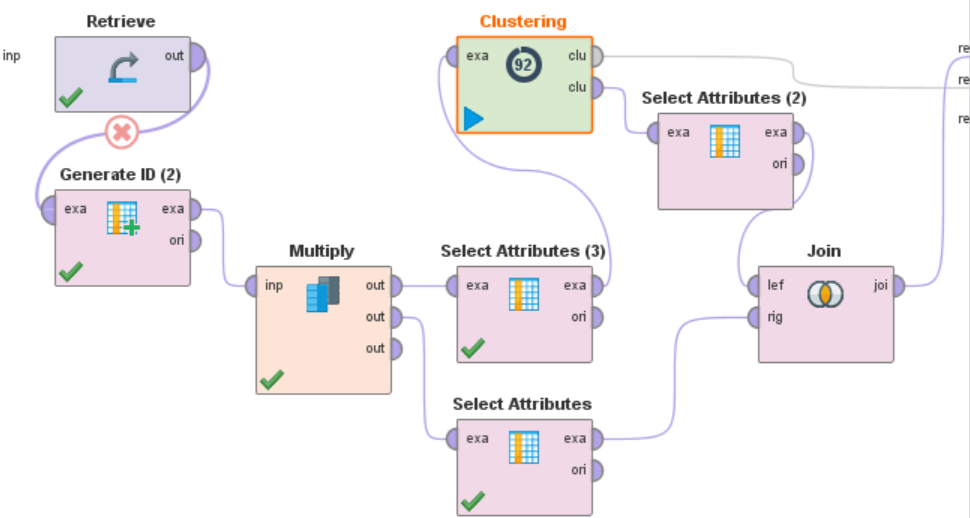
\includegraphics[width=0.9\textwidth]{ClusteringRapid.PNG}
\caption{Process of k-means clustering}
\label{fig: kclust}
\end{figure}


The Process, figure \ref{fig: kclust} contains the following steps:
\begin{description}
	\item[Retrieve] gives the data into the process. 
  \item[Generate ID] creates an ID such that we can make the comparsion step at the end through joining the sets
  \item[Multiply] creates two identical data sets
  \item[Select Attrbiutes] thoughs away the strata before the clustering step, everything behalve cluster and id after the clustering and just keeps id and strata for the join step
	\item[Clustering] runs the k-means clustering algorithm. The number of Clusters has to be fixed.
	\item[Join] For comparing the clustering result and the strata we join the two filtered data sets by the id
\end{description}

In the clustering block we can chose between different distance measures and maximal step numbers. We decided to concentrate on almost everywhere basic configurations and chose the squared euclidean distance in the mixed version.

In the first step we tried to cluster the \textbf{Original Data} in \textbf{6 Cluster}. Therefore we retrieved the original data set in RapidMiner and chose k as 6.

\ref{fig:OrgDist}. 
\begin{figure}[!htbp]
\centering
\begin{subfigure}{.5\textwidth}
  \centering
  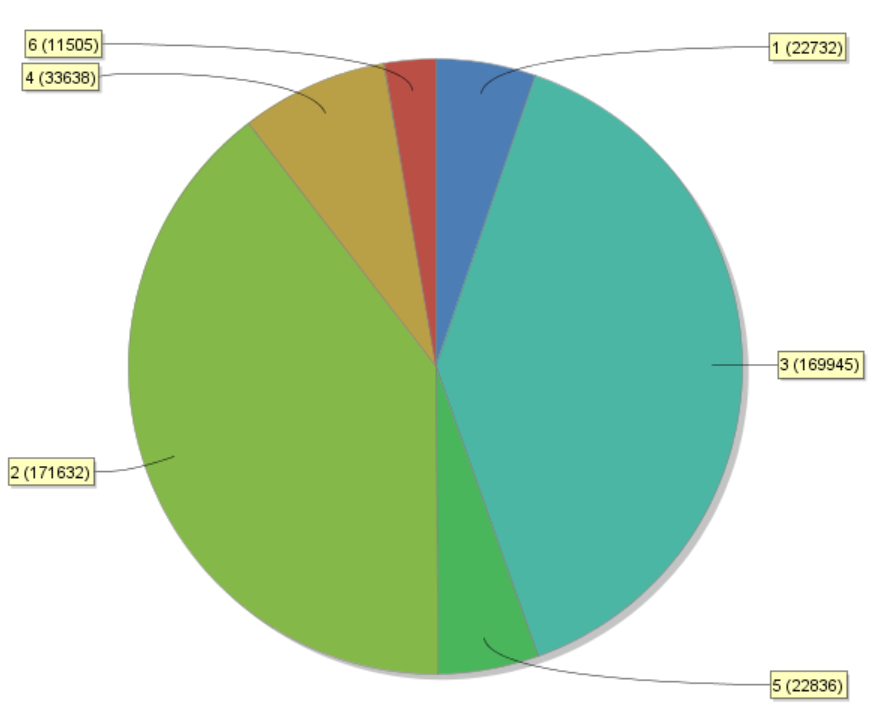
\includegraphics[width=.4\linewidth]{ClusterOrigRapidStrata.PNG}
  \caption{Strata}
  \label{fig:OrgSt}
\end{subfigure}%
\begin{subfigure}{.5\textwidth}
  \centering
  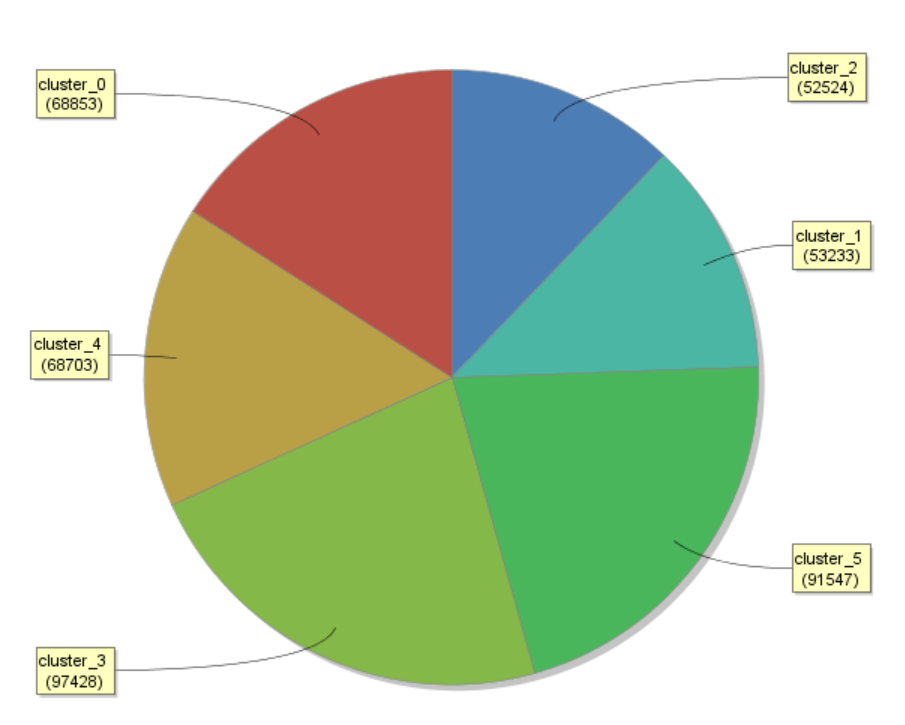
\includegraphics[width=.4\linewidth]{ClusterOrigRapidCluster.PNG}
  \caption{Cluster}
  \label{fig:OrgCl}
\end{subfigure}
\caption{Distribution of original data}
\label{fig:OrgDist}
\end{figure}

In figure \ref{fig:OrgDist} is the result to see of the first try. Figure \ref{fig:OrgSt} shows the strata distribution as pie chart and \ref{fig:OrgCl} the resulted cluster distribution. It can already been seen, that the distributions are not similar. In the next step we tried it with more steps, but the result was not looking better.

We asked ourselfs, if 6 cluster is not too fine, so we searched for \textbf{3 clusters} in the next step. The idea is to combine two stratas in 1, such that we just have 3 stratas left.
\begin{figure}[!htbp]
\centering
\begin{subfigure}{.5\textwidth}
  \centering
  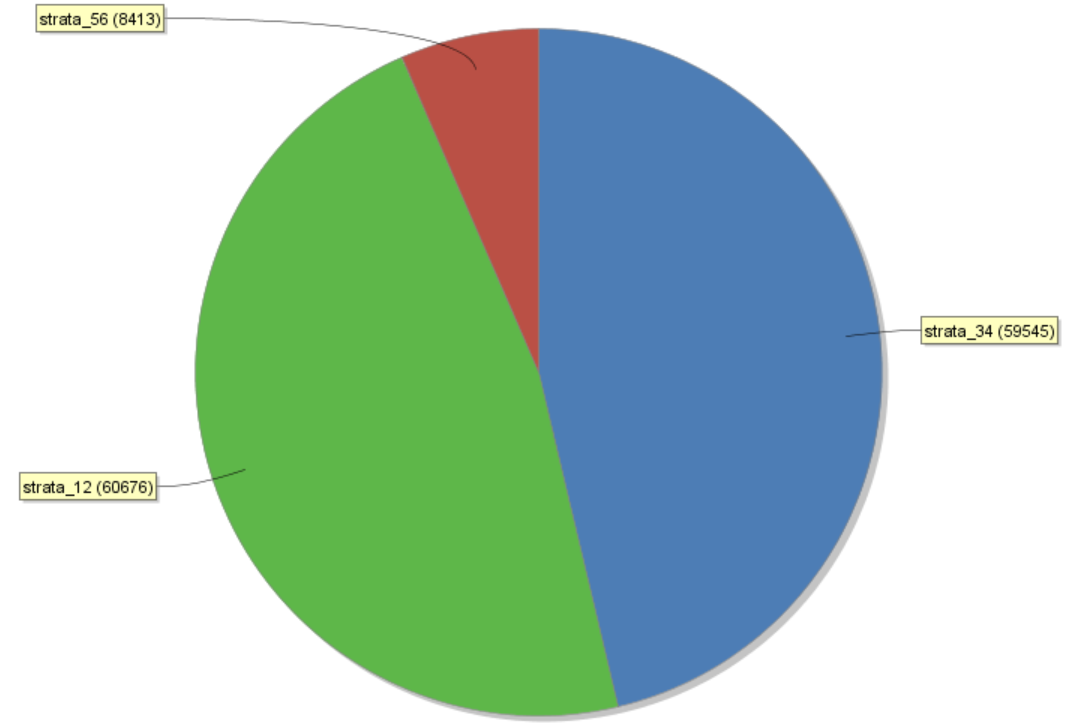
\includegraphics[width=.4\linewidth]{ClusterOrigRapidStrata2Cluster.PNG}
  \caption{Strata}
  \label{fig:OrgSt}
\end{subfigure}%
\begin{subfigure}{.5\textwidth}
  \centering
  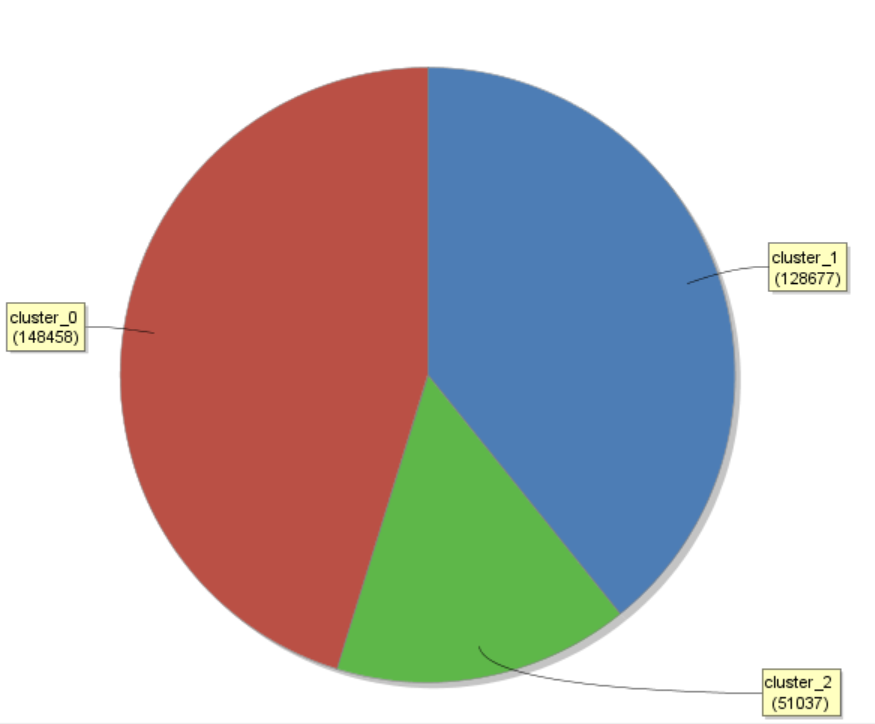
\includegraphics[width=.4\linewidth]{ClusterOrigRapidCluster2Cluster.PNG}
  \caption{Cluster}
  \label{fig:OrgCl}
\end{subfigure}
\caption{Distribution of original data}
\label{fig:OrgDist}
\end{figure}

Also the distribution in the strata groups of the clustering shows, that there is no real connection of strata and the clustering.
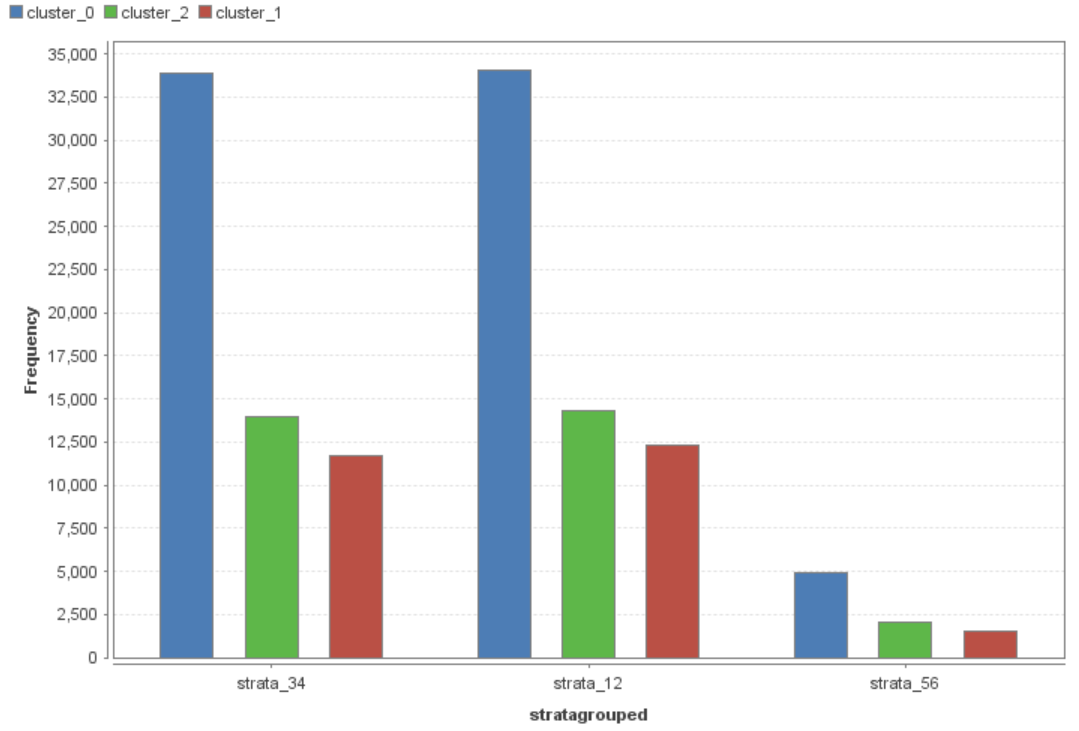
\includegraphics[width=0.9\textwidth]{ClusterOrigRapidDistribution2Cluster.PNG}

\subsection{Combined Data}

Because of the not really convincing result of the clustering like above we had the idea to combine for every ID the different pathes in one big vector. This garants us, that one person just can be in one cluster aswell. The idea is to sum up all pathes in one big vector.
\subsubsection{Code}
%hier darfst du dich gerne verewigen Timo. Gerne auch vorher und nachher noch mehr schreiben. Titel darf auch geändert werden
% boa das ist voll liep un soo weischt :D

Instead of simple IDs for every person we expand the parsing by using a data encapsulating in a class called \texttt{Person}. This class stores the ID, the parameters defining a person %TODO: ref zu code basics
, and all movements from that person.\\
Then we are able to compute the following vector, with 848 entries, for further usage, that combines all movements of the person:
$$\underbrace{\#o_1, \dots, \#o_{413}, \#d_1, \dots, \#d_{413}}_{2\cdot 413} ,
 \underbrace{\mathit{AM}, \mathit{MD}, \mathit{PM}, \mathit{MN}}_{4}, 
 \underbrace{\#r_1, \dots, \#r_7}_{7}, 
 \underbrace{\#\mathit{MoT}_1, \dots, \#\mathit{MoT}_7}_{7}, 
 \underbrace{\mathit{SD}, \mathit{SS}, \mathit{G}, \mathit{A}}_{4}$$
with the following abbreviations ($1 \le i \le 413$, $0 \le j \le 7$):
\begin{multicols}{2}
\begin{itemize}
	\item[$o_i$:]  the $i$-th origin data point
	\item[$d_i$:]  the $i$-th destination data point
	\item[$\mathit{AM}$:] movements at time stamp AM
	\item[$\mathit{MD}$:] movements at time stamp MD
	\item[$\mathit{PM}$:] movements at time stamp PM
	\item[$\mathit{MN}$:] movements at time stamp MN
	\item[$r_j$:] the $j$-th reason
	\item[$\mathit{MoT}_j$:] the $j$-th mean of transportation
	\item[$\mathit{SD}$:] sum of all durations
	\item[$\mathit{SS}$:] sum of all distances
	\item[$\mathit{G}$:] the gender
	\item[$\mathit{A}$:] the age
\end{itemize}
\end{multicols}

\subsubsection{Searching for 6 Clusters}
Applying the process with maximal 100 steps on the data gives us the following results.

Like above we check first the total distribution of strata and clusters with a pie. You already see, that it is not the 
\begin{figure}[h]
\centering
\begin{subfigure}{.5\textwidth}
  \centering
  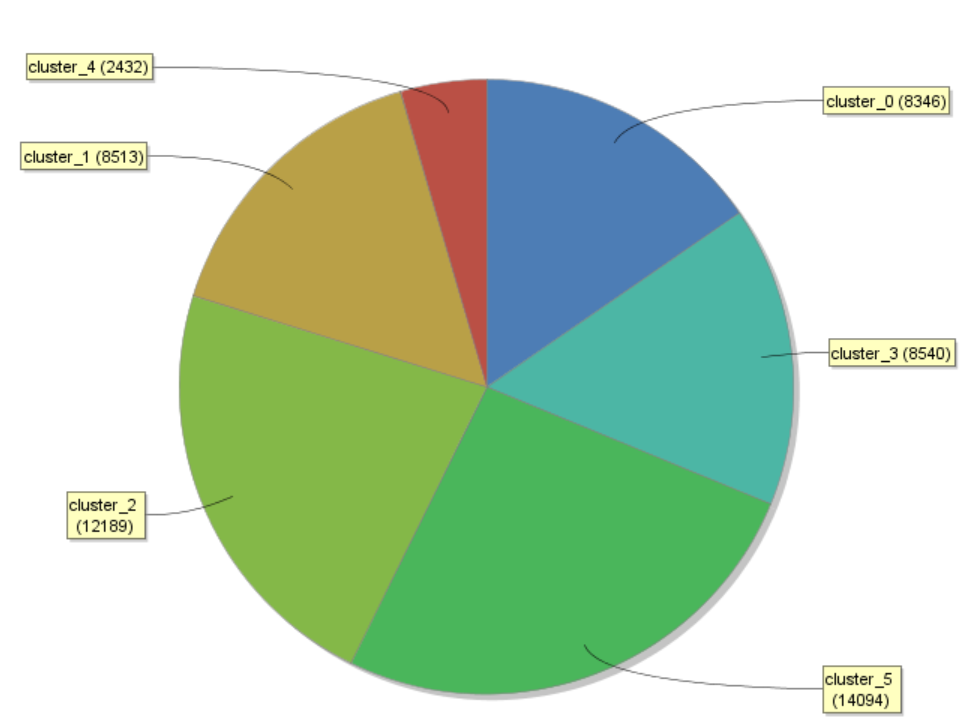
\includegraphics[width=.4\linewidth]{vectorclusteringcluster.PNG}
  \caption{Strata}
  \label{fig:OrgSt}
\end{subfigure}%
\begin{subfigure}{.5\textwidth}
  \centering
  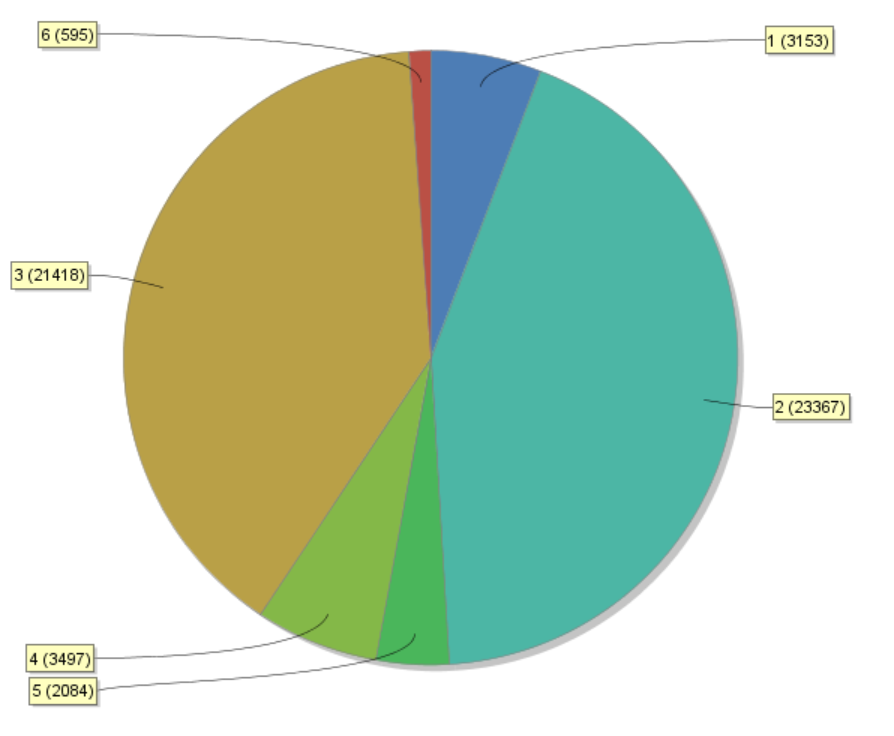
\includegraphics[width=.4\linewidth]{vectorclusteringstrata.PNG}
  \caption{Cluster}
  \label{fig:OrgCl}
\end{subfigure}
\caption{Distribution of original data}
\label{fig:OrgDist}
\end{figure}

Also the distribution in the strata groups of the clustering shows, that there is not really a connection of strata and the clustering to see.
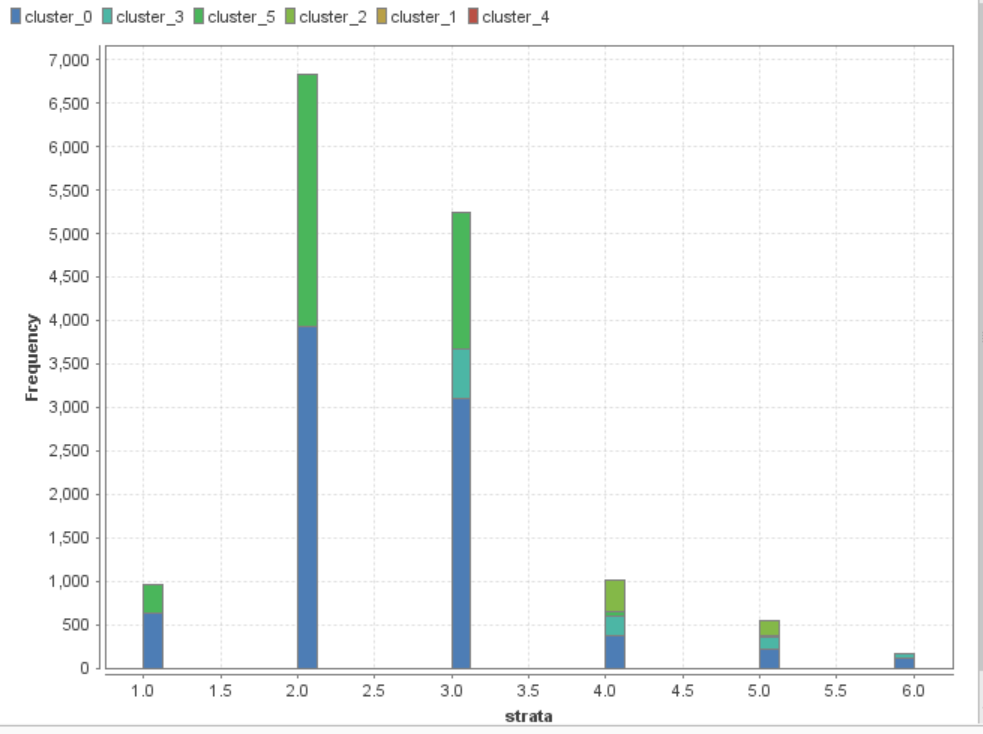
\includegraphics[width=0.9\textwidth]{vectorClustering.PNG}

So we change the maximal stepsize to 1000 and let the algorithm run again.

\begin{figure}[h]
\centering
\begin{subfigure}{.5\textwidth}
  \centering
  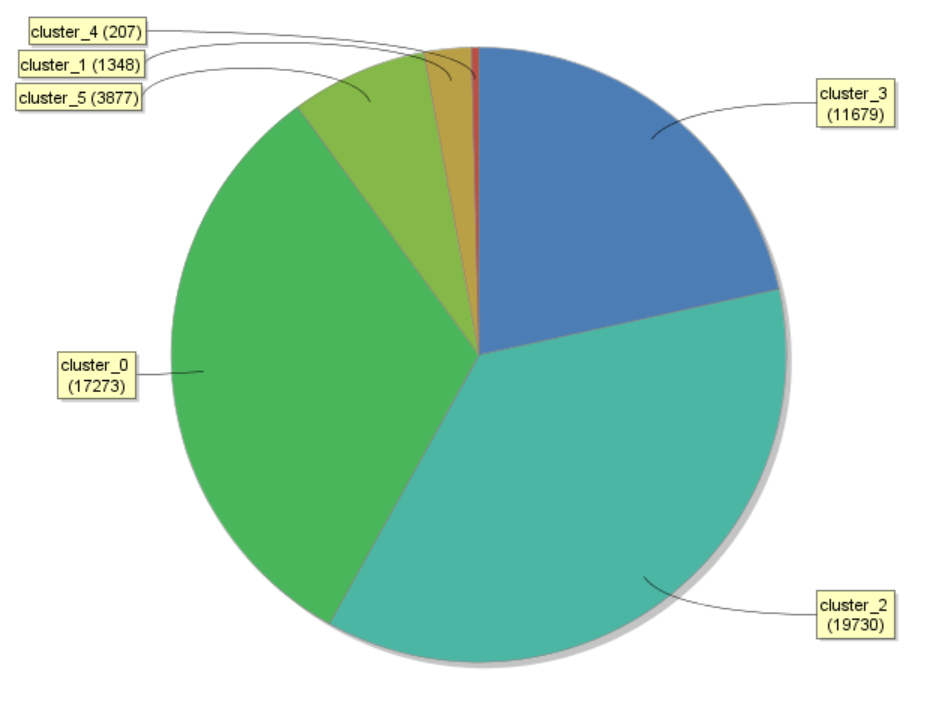
\includegraphics[width=.4\linewidth]{vectorclusteringcluster1000.PNG}
  \caption{Strata}
  \label{fig:OrgSt}
\end{subfigure}%
\begin{subfigure}{.5\textwidth}
  \centering
  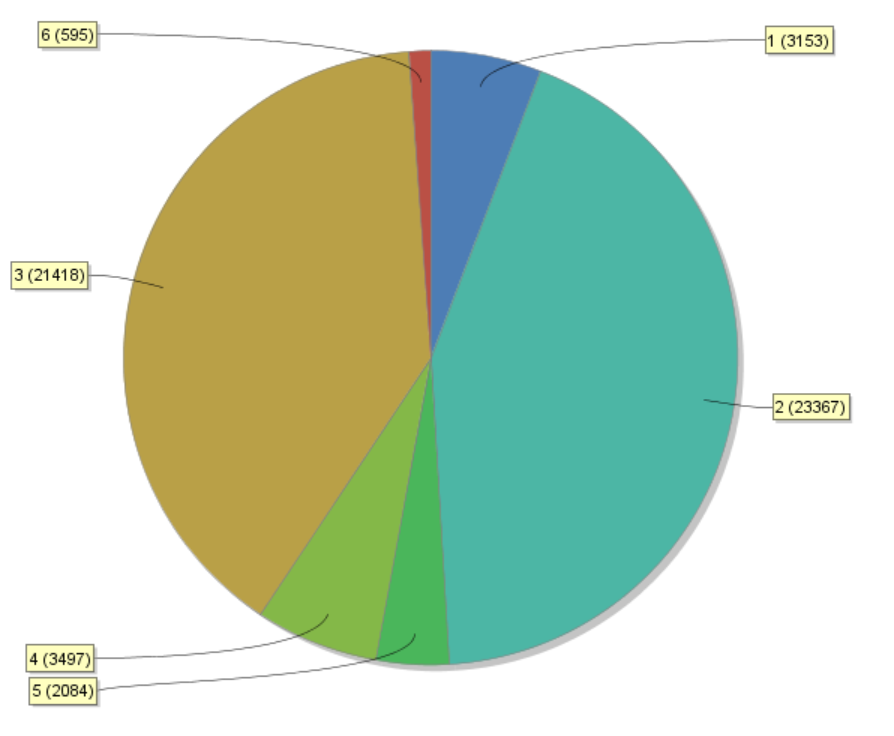
\includegraphics[width=.4\linewidth]{vectorclusteringstrata.PNG}
  \caption{Cluster}
  \label{fig:OrgCl}
\end{subfigure}
\caption{Distribution of original data}
\label{fig:OrgDist}
\end{figure}

So we already get the idea, that there are not 6 Clusters, but just 3. Checking the distribution still gives us no strong correlation between strata and cluster.

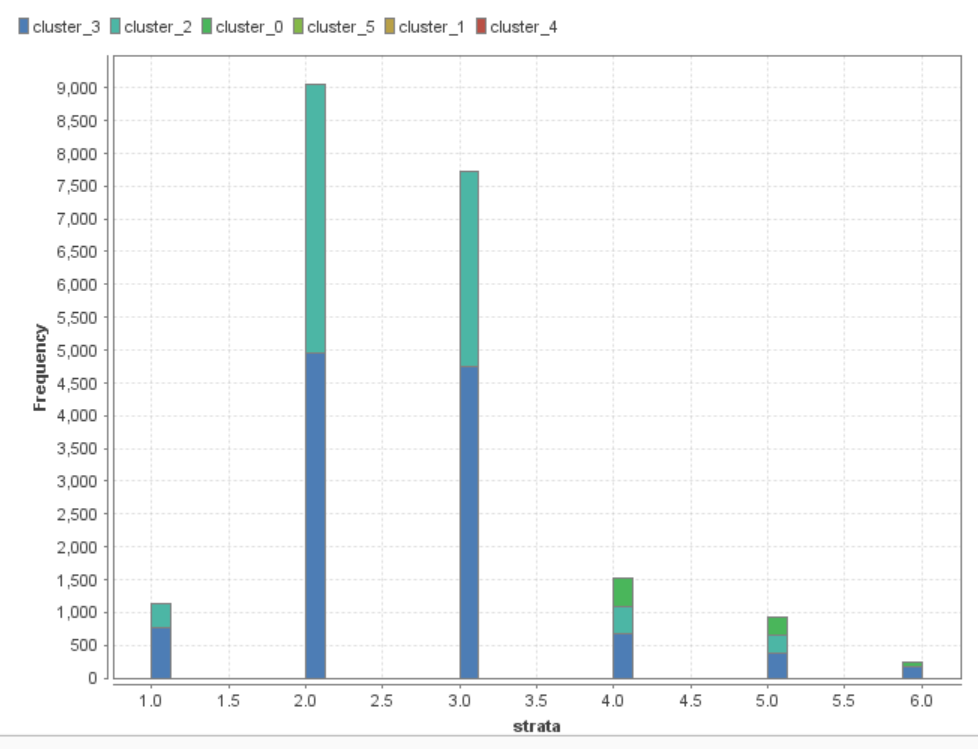
\includegraphics[width=0.9\textwidth]{vectorClustering1000}

\subsubsection{Searching for 3 Clusters}

Because of the result in the last part, we checked the behavior of the clustering by just searching for 3 Cluster. The first try is with 100 steps again.

\begin{figure}[h]
\centering
\begin{subfigure}{.5\textwidth}
  \centering
  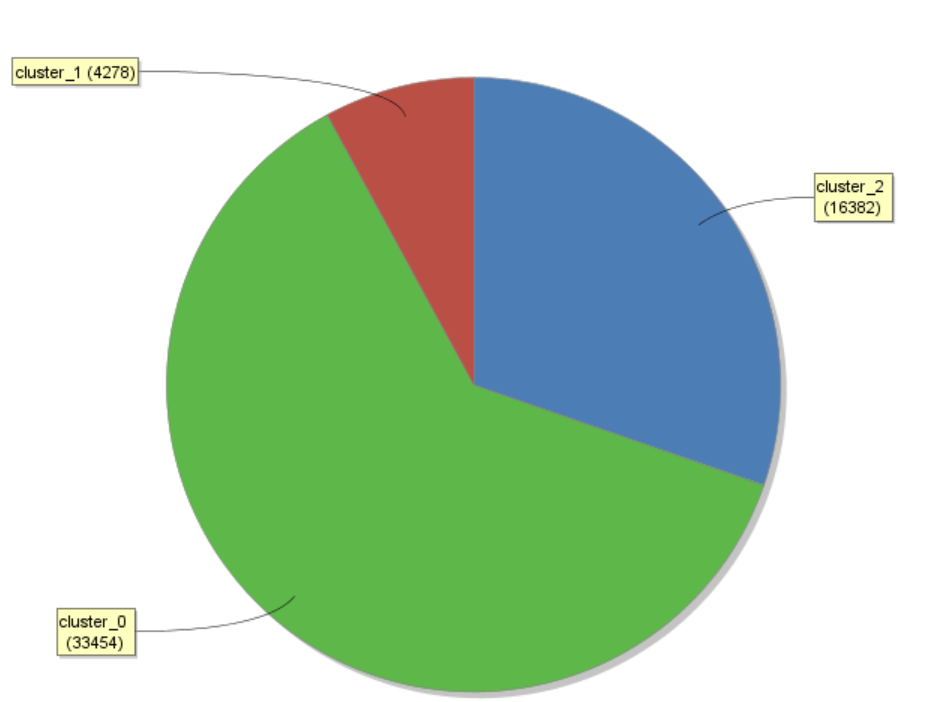
\includegraphics[width=.4\linewidth]{vectorclusteringcluster3Cluster.PNG}
  \caption{Strata}
  \label{fig:OrgSt}
\end{subfigure}%
\begin{subfigure}{.5\textwidth}
  \centering
  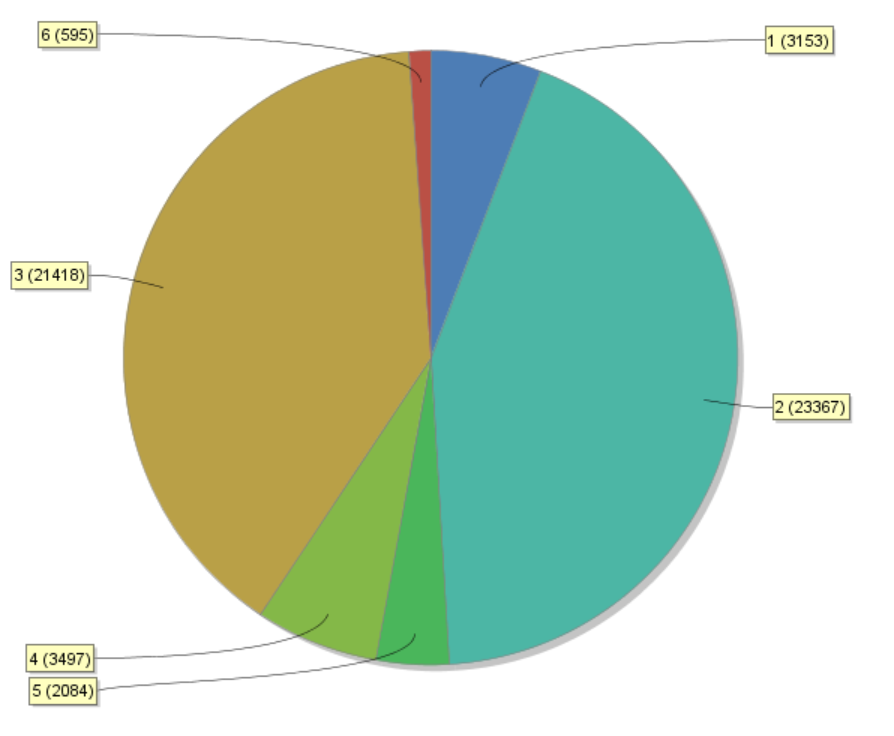
\includegraphics[width=.4\linewidth]{vectorclusteringstrata.PNG}
  \caption{Cluster}
  \label{fig:OrgCl}
\end{subfigure}
\caption{Distribution of original data}
\label{fig:OrgDist}
\end{figure}

This comes closer by the orginial distribution combining two stratas in one cluster.

But having a look at the inbetween distribution does not show us a real correlation between cluster and strata.

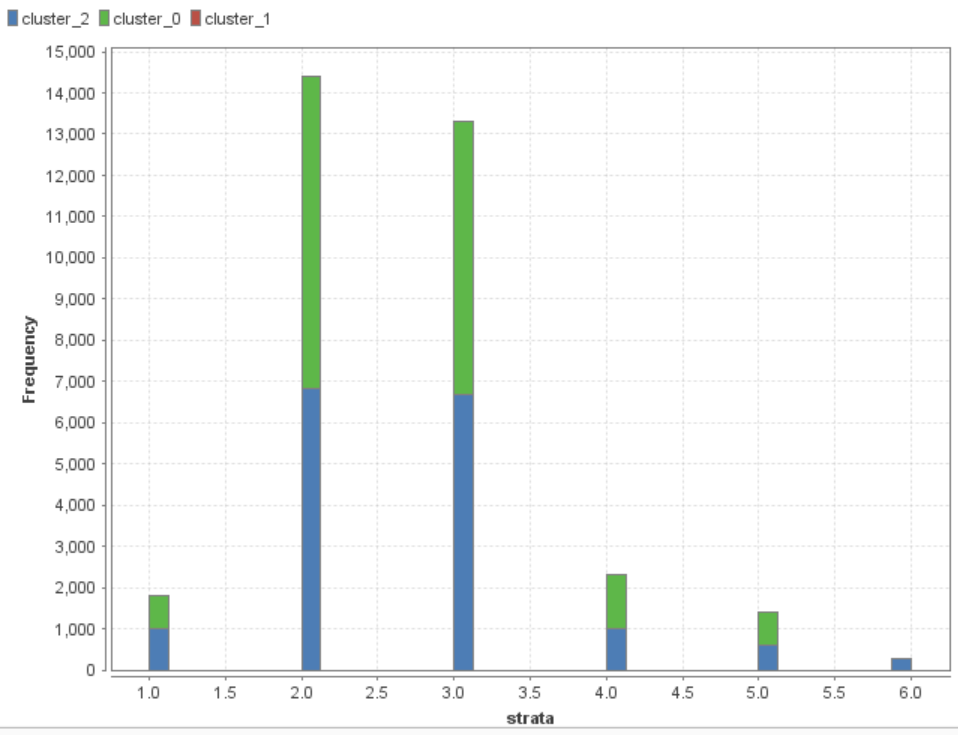
\includegraphics[width=0.9\textwidth]{vectorClustering3Cluster.PNG}

We wanted to check what happens when giving the process 1000 steps maximal. 